\subsection{Framework Overview}

Our framework is shown in Fig.~\ref{fig:framework}.
It is a general approach that can be incorporated into most of the previous RL-based Locomotion methods such as RMA~\cite{kumar2021rma}, Dreamwaq~\cite{nahrendra2023dreamwaq}, HIMLoco~\cite{long2024him}, etc., and here we use HIMLoco as the backbone algorithm.
It consists of two parts: Motion Reference Learning and Policy Learning with Imagined Transition.
Section~\ref{sec4_1} discusses how to perform Motion Reference Learning. It aims to obtain the optimal gait from a fixed simulation environment and compress the optimal gait into an ideal policy and a dynamics model.
Section~\ref{sec4_2} presents how to use motion reference to guide policy learning.


\subsection{Motion Reference Learning in Fixed Dynamics}
\label{sec4_1}
\subsubsection{Ideal Policy}
In the process of reinforcement learning to train robotic policies, we found that the wider ranges of dynamic randomization, the lower returns that can be obtained when the training converges.
To obtain an optimal reference, we train a policy that is optimal in the unperturbed simulation environment in a fixed dynamic (i.e., no dynamic randomization setting) environment, which is called the ideal policy $ \pi_{ideal}(\mathbf{a}^r_t|\mathbf{o}_{t:t-H}) $ in the paper.

\subsubsection{Dynamics Model}
\begin{figure}[h]
    \centering
    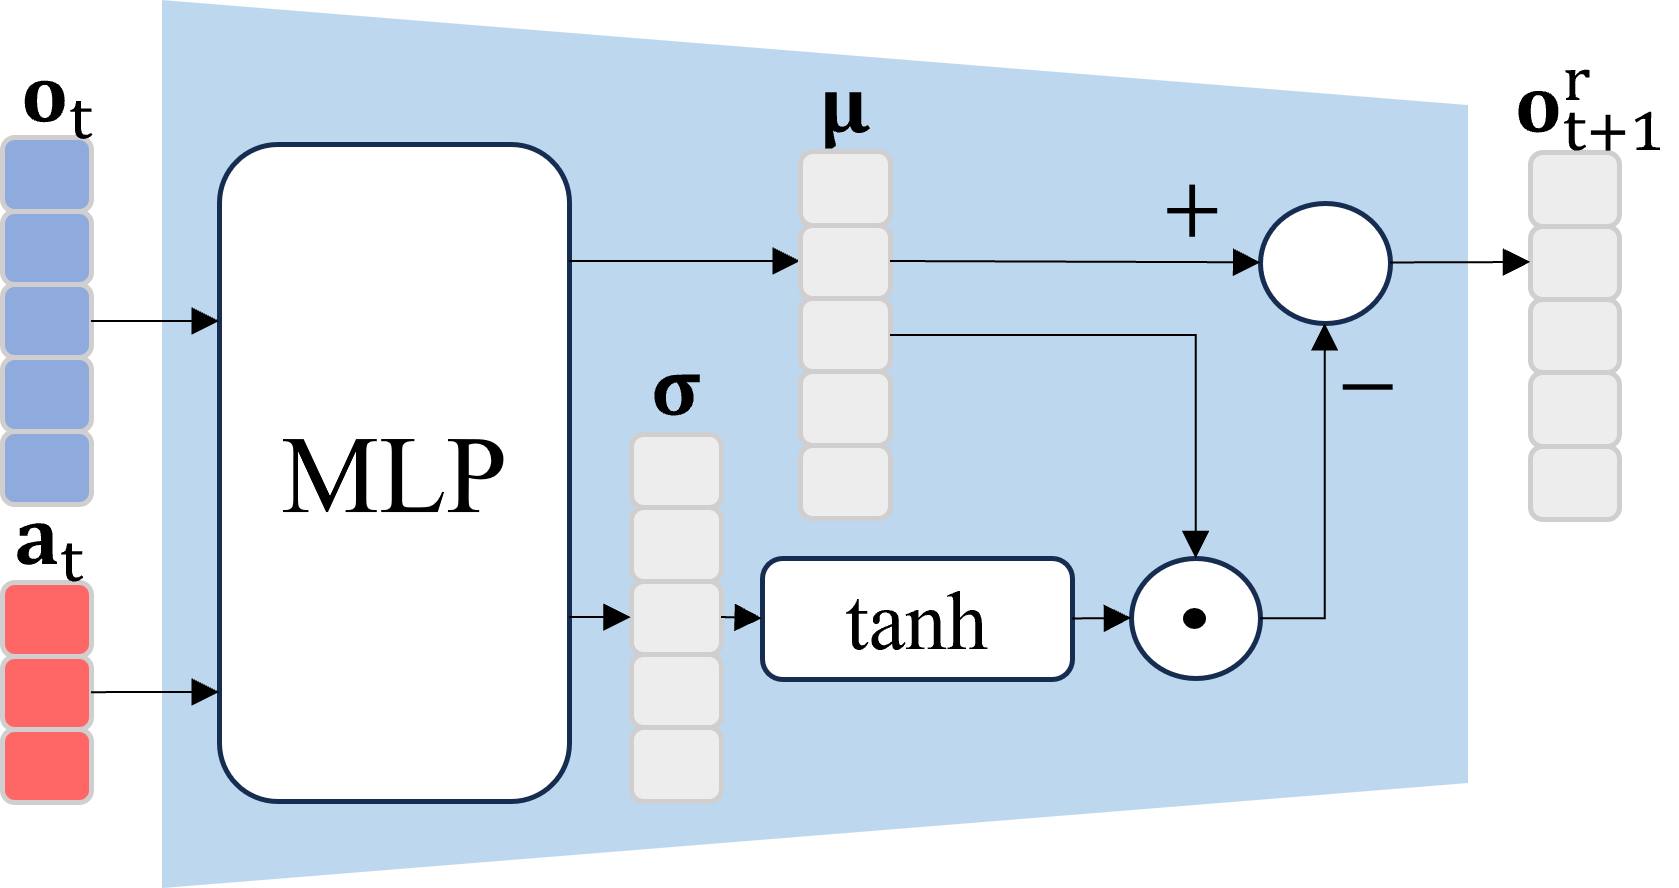
\includegraphics[width=0.8\linewidth]{fig/model.png}
    \caption{\textbf{Architecture of Dynamics Model.} An adjustment mechanism is added to the output of the dynamics model.}
    \label{fig:model}
\end{figure}
To obtain reference observations, we train a dynamics model under the non-perturbative simulation environment.
The output of the dynamics model includes $\mu$ and  $\sigma$ in eq.~\ref{eq:output}, which means the mean and standard deviation of the next observation estimation.
We use the dynamics model to output $\mu$ and $\sigma$, which parameterize a normal distribution. The training objective is to maximize the likelihood of the true next observation $\mathbf{o}_{t+1}$ under this distribution.

\begin{equation}
    \mu, \sigma = d_{\theta}(\cdot | \mathbf{o}_t, \mathbf{a}_t)
    \label{eq:output}
\end{equation}
\begin{equation}
    \mathcal{L}_{MLE} = -\mathbb{E}[\log p(\mathbf{o}_{t+1}|\mu,\sigma)]
    \label{eq:mle}
\end{equation}

In most model-based methods, model error is an unavoidable problem.
We measured prediction error  \( \|{\mathbf{o}}_{t+1} - \mu\|_2 \) while applying the unseen disturbance in the robot's body or not, and compared it to \( \sigma \).
The results in Fig.~\ref{fig:stdev} show a strong correlation between actual prediction error and $\sigma$ given by the learned model.

\begin{figure}[h]
    \centering
    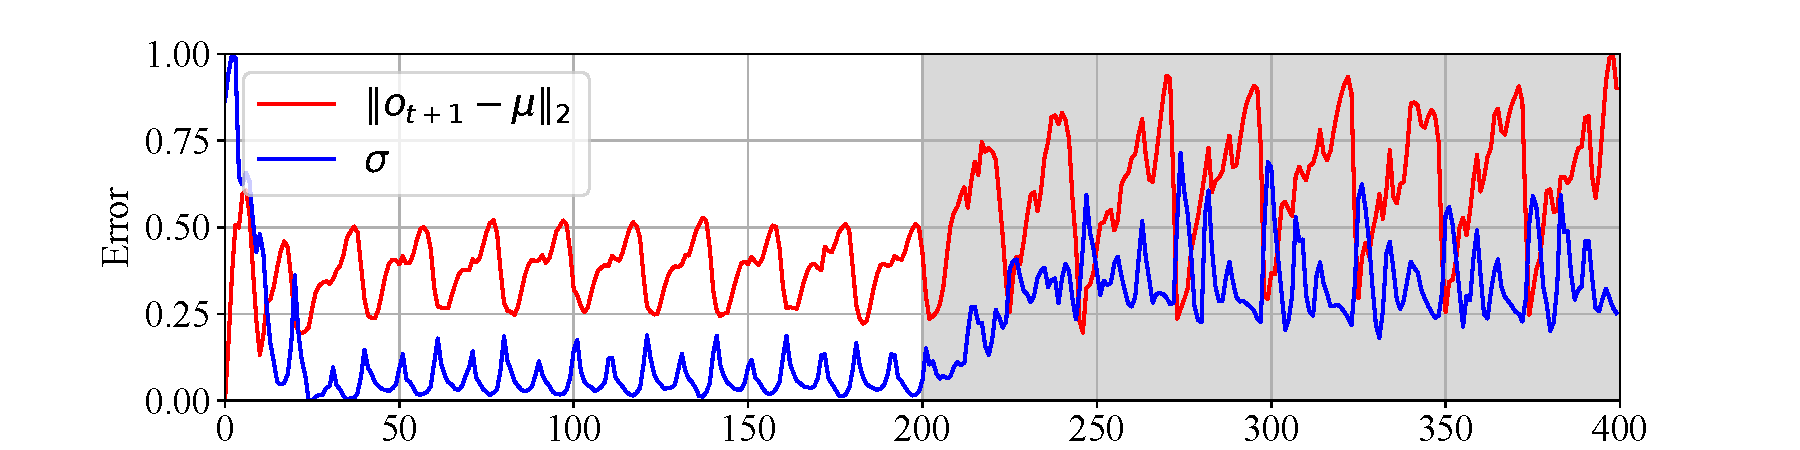
\includegraphics[width=1\linewidth]{fig/stdev.pdf}
    \caption{Correlation between standard deviation estimate and actual observation bias. Unseen disturbance is applied to the robot after 200 steps.}
    \label{fig:stdev}
\end{figure}

To prevent training and deployment collisions caused by model inaccuracies, we developed an adjustment mechanism to adjust the prediction of the next observation in the following robust policy learning stage (see Sec.~\ref{sec4_2}) and deployment.
According to the general law of supervised learning, the larger the standard deviation $\sigma$ the less reliable the prediction $\mu$ of the dynamics model.
Thus, when the variance is large, we should minimize the effect of the observation reference on the subsequent network. 
Inspired by~\cite{nahrendra2023dreamwaq, nahrendra2024obstacle}, we multiply the weight $(1- norm(\sigma)) \in [0, 1]$ dot by $\mu$ with the following equation~\ref{eq:adjust}.
Experiments in~\ref{fig:payload} showed that this design significantly improved the robot's performance in the unseen region.

\begin{equation}
    \mathbf{o}^{r}_{t+1} = (1- norm(\sigma))\cdot\mu
    \label{eq:adjust}
\end{equation}

\subsection{Policy Learning with Imagined Transition}
\label{sec4_2}
\begin{figure}[h]
    \centering
    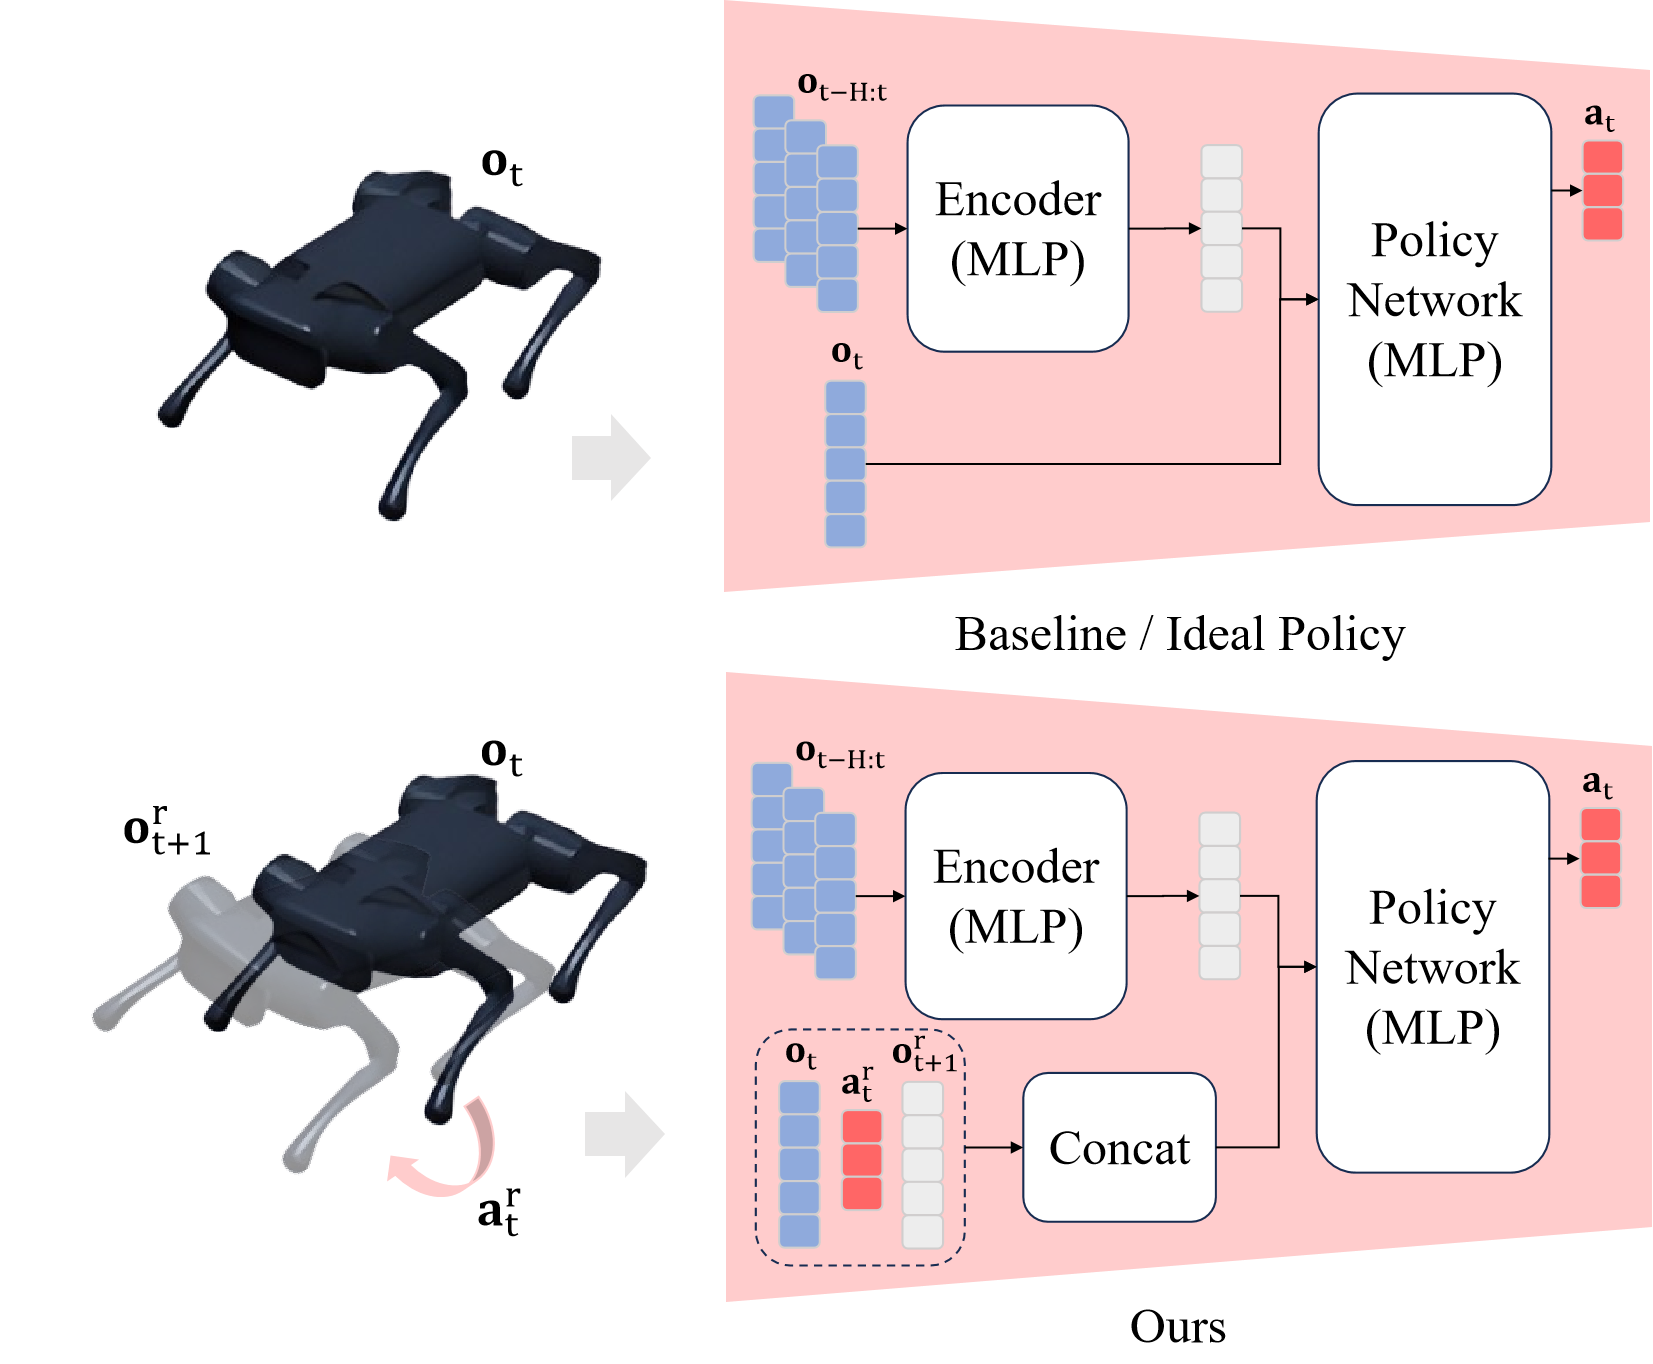
\includegraphics[width=0.9\linewidth]{fig/actor.png}
    \caption{\textbf{Architecture of Policy Network.} The top is the baseline architecture, and the bottom is the architecture of the policy network with imagined transition.}
    \label{fig:actor}
\end{figure}

In short, the only difference in our policy network is that we are adding the input of action and observation reference, which represents motion reference.
The combination of $\mathbf{o}_{t}$, $\mathbf{a}^{r}_{t}$, and $\mathbf{o}^{r}_{t+1}$ forms a complete state transition $\{\mathbf{o}_{t}, \mathbf{a}^{r}_{t}, \mathbf{o}^{r}_{t+1}\}$, which is our imagined transition.
As shown in the bottom of Fig.\ref{fig:actor}, we concatenate reference action $\mathbf{a}^{r}_{t}$ and imagined next observation $\mathbf{o}^{r}_{t+1}$ from the motion reference with proprioceptive observations $\mathbf{o}_{t}$, whereas the baseline, depicted on the top, follows the encoder-policy network architecture used in\cite{nahrendra2023dreamwaq, long2024him}.

\begin{equation}
    \mathbf{a}_t \sim \pi(\cdot | \mathbf{o}_{t-H:t})
\end{equation}
\begin{equation}
    \mathbf{a}_t \sim \pi(\cdot | \mathbf{o}_{t-H:t}, \mathbf{a}^{r}_{t}, \mathbf{o}^{r}_{t+1})
\end{equation}

% Intuitively, solving in the solution space close to the motion prior should be more efficient than searching for the optimal solution directly in the huge solution space.
% This simple change has resulted in a significant increase in the overall performance of policy learning.

We argue that while dynamics randomization hugely extend the solution space for robotic policies, it does not change the behavior robot should be. 
For instance, given a command to "move forward 1.0 meter," the policy is expected to execute exactly that distance across all randomized environments, rather than drifting to 0.9 or 1.1 meters.
The imagined transition $\{\mathbf{o}_{t}, \mathbf{a}^{r}_{t}, \mathbf{o}^{r}_{t+1}\}$ represents the desired behavior established in the previous RL \ref{sec4_1}. By leveraging it, policy optimization becomes more efficient than searching for the optimal solution directly in the huge solution space.